\documentclass[conference]{IEEEtran}
\usepackage[T1]{fontenc}
\usepackage{amsmath,amssymb,graphicx,booktabs,tabularx,array,url}
\usepackage[hidelinks]{hyperref}
\newcolumntype{Y}{>{\raggedright\arraybackslash}X}
\title{Photovoltaic Data Preprocessing and Feature Engineering:\\An Empirical Strategy-to-Execution Audit}
\author{\IEEEauthorblockN{Ruganji Prince}
\IEEEauthorblockA{Carnegie Mellon University Africa\\04-652 Artificial Intelligence System Design\\Assignment 3: Data Preprocessing Phase 2}}
\begin{document}
\maketitle
\begin{abstract}
This reflection executes and audits a photovoltaic measurement preprocessing strategy using the released 1,373,798-row dataset. The workflow retains suspicious observations, isolates learned statistics to the training partition, and implements target-free transformations through Scikit-Learn Pipeline and ColumnTransformer. Eight diagnostic figures support numerical checks of missingness, distributions, collinearity, target association, scaling and exploratory PCA. The six-channel reference produces twelve mathematical inputs with availability indicators; alternative representations are documented without a predictive comparison. No classifier is fitted and no deployment-performance conclusion is drawn.
\end{abstract}
\begin{IEEEkeywords}
Photovoltaic measurements, preprocessing, feature engineering, data quality, leakage prevention, mutual information, PCA.
\end{IEEEkeywords}

\section{Scope, Data and Source Audit}
The current milestone is data preprocessing and feature engineering. The original-author dataset~\cite{dataset} and associated monitoring study~\cite{study} provide two provisionally aligned source vectors. The immutable CSV preserves exported source order and contains $N=1{,}373{,}798$ observations and $P=7$ variables: six continuous predictors and nominal target $f\_nv$ (Table~\ref{tab:data}). Voltage/current quantities are source-described DC RMS measurements; module temperature aggregates source probes. Integer target codes are labels, not an ordinal or continuous measurement.

The study describes nominal 1\,Hz acquisition, per-second electrical RMS calculations, one-second irradiance/temperature averages and a 16-day experiment. Released arrays contain no timestamp. Absolute time and uninterrupted one-second spacing cannot be reconstructed. Sixteen signal-defined blocks are therefore not verified days, sessions or hours. All references to positions describe export order only.

The raw class counts are 1,162,931 / 5,999 / 10,371 / 6,024 / 188,473 for normal / short circuit / resistive degradation / open circuit / natural building shade. Filtering $irr\geq100\,\mathrm{W/m^2}$ yields 515,958 rows and the literature counts 309,253 / 5,999 / 10,371 / 6,024 / 184,311 exactly. This suggests a possible evaluation-population explanation, but the study does not explicitly document that exact filter. Low-irradiance values are not all labeled nighttime, and no rows are removed to force agreement with the paper.
\begin{table}[!t]
\caption{Raw schema and exported missingness (all rows).}\label{tab:data}
\centering\footnotesize
\begin{tabularx}{\columnwidth}{Yrr}
\toprule
Variable / role & Unit & Missing \\ \midrule
\texttt{vdc1}, \texttt{vdc2}: continuous predictors & V & 0 (0\%) \\
\texttt{idc1}, \texttt{idc2}: continuous predictors & A & 0 (0\%) \\
\texttt{irr}: continuous predictor & $\mathrm{W/m^2}$ & 0 (0\%) \\
\texttt{pvt}: continuous predictor & $^\circ$C & 0 (0\%) \\
\texttt{f\_nv}: nominal target & --- & 0 (0\%) \\
\bottomrule
\end{tabularx}
\end{table}

\section{Quality, Missingness and Outlier Decisions}
\subsection{Missingness and suspicious values}
The implementation audits the approved Phase 1 strategy~\cite{phase1} against executed preprocessing evidence.
Figure~\ref{fig:missing} displays a seed-42 uniform sample of 5,000 TRAIN positions. The full release has zero conventional missing cells out of 9,616,586 (0\%); all 1,373,798 rows are complete. MCAR/MAR/MNAR inference from observed missingness is not applicable: neither Little's MCAR test nor missing-indicator Cramer's V is meaningful with a constant, all-observed mask. Unrecorded intervals remain unobservable. No missingness mechanism is inferred from zero NaNs.

The 62 paired $irr=0,pvt=0$ observations occur in runs of 1/32/29 and remain suspicious observations rather than confirmed missing values. The source does not establish zero as a missing sentinel. One irradiance value is $-0.0381\,\mathrm{W/m^2}$; the predeclared convention clamps $-1\leq irr<0$ to zero only in processed matrices. Values below $-1$ and negative electrical measurements would become unavailable. All 24,172 released negative-Celsius observations remain valid candidates; TRAIN temperature reaches $-1.6543\,{}^\circ$C (Table~\ref{tab:outliers}). The raw CSV remains unchanged.

TRAIN-median contingency imputation and per-retained-channel availability indicators are retained. There are no exported NaNs requiring ordinary imputation. A median is less sensitive to extremes than a mean, but a low-light median can still be unsuitable during generation. Mode is unsuitable for continuous measurements; KNN adds distance and computational assumptions; interpolation requires continuity not established here. Eligibility flags allow at most one unavailable retained channel for at most two consecutive source positions, resetting at gaps/block boundaries; all arrays preserve row alignment.

\subsection{Distribution-qualified screening rather than forced capping}
Figure~\ref{fig:outliers} compares raw with reference-cleaned TRAIN measurements. The audit uses $[Q_1-1.5\,IQR,Q_3+1.5\,IQR]$ and a complementary distribution-qualified $|Z|>3$ screen. Table~\ref{tab:outliers} reports the actual fences, skewness and unbiased Fisher excess kurtosis. Every predictor has zero IQR flags (0\%) and zero $|Z|>3$ flags under the retained full-TRAIN reference. Negative excess kurtosis and multi-regime mixtures do not justify a Gaussian assumption. In particular, current/irradiance mean--median differences show why no universal mean-filling rule is asserted.

No automatic statistical capping or row deletion is selected. Broad full-population fences are screens, not physical-validity certificates; rare fault-state measurements may carry genuine information. Nearly identical panels in Fig.~\ref{fig:outliers} are expected, not evidence of a failed cleaning operation. The only observed quality change is the one near-zero irradiance clamp. This deterministic engineering convention changes one processed value and is not claimed to be literally lossless; its original value remains recoverable in the immutable export.

\section{Relationships, Relevance and Feature Retention}
Figure~\ref{fig:target} shows all TRAIN labels at natural prevalence: 844,805 / 1,226 / 5,695 / 1,204 / 153,199, with normal representing 83.9659\%. No target encoding as a continuous quantity, synthetic oversampling or row duplication is introduced. No categorical predictor requires ordinal or one-hot encoding. Nominal-target association is separated from predictor--predictor correlation.

Figure~\ref{fig:correlation} is the upper-triangle six-predictor TRAIN Pearson matrix; $f\_nv$ is excluded. Table~\ref{tab:pairs} lists all five pairs with $|r|\geq0.85$. Figure~\ref{fig:scatter} displays a uniform seed-42 sample of 20,000 TRAIN positions; correlations and descriptive OLS lines use full TRAIN. Spearman is a possible sensitivity method, not an unperformed result claimed in this report. Association does not imply significance or causation under dependent repeated readings.

The original TRAIN VIF values are independently checked as the diagonal of the inverse centered Pearson matrix, equivalent to intercept-OLS VIF. Five values exceed 10 (Table~\ref{tab:association}), confirming strong dependence without proving physical redundancy. All six reference inputs are retained; VIF/correlation alone does not select a physical-channel removal.

Figure~\ref{fig:mi} is \emph{Target Association / Mutual Information Feature Screening}, not trained-model feature importance. Continuous-predictor/nominal-target MI uses a seed-42 proportional stratified sample of 50,000 TRAIN observations, $k=3$, and TRAIN-fitted standardization. Sample counts are 41,983 / 61 / 283 / 60 / 7,613. Table~\ref{tab:association} gives the scores in nats. Imbalance, ties and dependent rows limit interpretation. These descriptive scores do not trigger predictor deletion or establish causal sensor importance.
\begin{table*}[!t]
\caption{TRAIN distribution and outlier audit, before reference cleaning. $N=1{,}006{,}129$ per predictor. All IQR and $|Z|>3$ counts are zero; excess kurtosis is unbiased Fisher kurtosis.}\label{tab:outliers}
\centering\footnotesize
\begin{tabularx}{\textwidth}{Yrrrrrrr}
\toprule
Predictor & $Q_1$ & $Q_3$ & IQR & Lower & Upper & Skew & Excess kurt. \\ \midrule
vdc1 & 1.0184 & 274.4720 & 273.4536 & -409.1620 & 684.6524 & 0.0683 & -1.9302 \\
vdc2 & 0.9824 & 272.3780 & 271.3956 & -406.1110 & 679.4714 & 0.0909 & -1.8973 \\
idc1 & 0.0648 & 4.9670 & 4.9022 & -7.2885 & 12.3203 & 1.0046 & -0.6707 \\
idc2 & 0.0088 & 4.0011 & 3.9923 & -5.9797 & 9.9896 & 1.1450 & -0.3666 \\
irr & 1.2889 & 586.3810 & 585.0921 & -876.3492 & 1464.0192 & 0.8745 & -0.9456 \\
pvt & 12.5516 & 34.0299 & 21.4783 & -19.6658 & 66.2473 & 0.5157 & -0.6303 \\
\bottomrule
\end{tabularx}
\end{table*}
\begin{table}[!t]
\caption{Five flagged TRAIN predictor pairs. Full-TRAIN values support Figs.~\ref{fig:correlation}--\ref{fig:scatter}.}\label{tab:pairs}
\centering\footnotesize
\begin{tabularx}{\columnwidth}{Yr}
\toprule
Predictors & Pearson $r$ \\ \midrule
vdc1 / vdc2 & 0.989103 \\
idc1 / idc2 & 0.952833 \\
idc1 / irr & 0.979472 \\
idc1 / pvt & 0.862289 \\
idc2 / irr & 0.955982 \\
\bottomrule
\end{tabularx}
\end{table}
\begin{table}[!t]
\caption{TRAIN-only VIF verification and descriptive nominal-target MI. MI uses a proportional 50,000-observation sample, not model-based importance.}\label{tab:association}
\centering\footnotesize
\begin{tabularx}{\columnwidth}{Yrr}
\toprule
Predictor & VIF & MI (nats) \\ \midrule
vdc1 & 52.168202 & 0.178615 \\
vdc2 & 56.345662 & 0.220611 \\
idc1 & 31.495610 & 0.276227 \\
idc2 & 15.780847 & 0.276981 \\
irr & 39.292651 & 0.300592 \\
pvt & 4.069798 & 0.112375 \\
\bottomrule
\end{tabularx}
\end{table}

\section{Scaling and Exploratory Dimensionality}
Figure~\ref{fig:scaling} compares the existing raw, StandardScaler, RobustScaler and MinMaxScaler irradiance representations. The standardized six-input reference supports scale-sensitive later methods; native-scale alternatives remain documented separately. Standardization aligns units/penalties rather than asserting Gaussian input. Table~\ref{tab:scaling} records actual TRAIN behavior. Across all six standardized channels, absolute means are below $10^{-10}$ and population standard deviations are one within $10^{-10}$.

The irradiance median is 1.8733 while the raw mean is 257.9285\,W/m$^2$. Robust scaling centers the median at zero and maps its IQR to one; MinMax maps the quality-processed TRAIN range to [0,1]. Held-out values are not guaranteed to stay within [0,1]. Positive affine scaling leaves skewness effectively unchanged at 0.8745; the tiny raw-versus-processed difference reflects the single near-zero quality clamp. No log transform was selected or added merely to reproduce an illustrative assignment example. Robust/MinMax are diagnostic alternatives, not a retrospective replacement of the reference preprocessing.

Figure~\ref{fig:pca} includes individual/cumulative variance and both 90\% and 95\% cutoffs. Full-SVD PCA fits a TRAIN-only standardized six-column matrix; covariance eigenvalues are independently verified (Table~\ref{tab:pca}). PC1 explains 82.5301\%; the first two explain 95.1677\%, crossing both cutoffs. A two-component diagnostic view omits 4.8323\% of variance and is not described as lossless. PCA is not selected in the primary pipeline. All six measured inputs remain necessary to compute its components, so two mathematical components do not mean two physical sensors.
\begin{table*}[!t]
\caption{TRAIN irradiance scaling behavior (population standard deviation). Values follow quality processing except the raw row.}\label{tab:scaling}
\centering\footnotesize
\begin{tabularx}{\textwidth}{Yrrrrrr}
\toprule
Representation & Mean & Std. & Median & Min. & Max. & Skew \\ \midrule
raw & 257.928481 & 349.018335 & 1.873300 & -0.038100 & 1085.920000 & 0.874462 \\
standard & -0.000000 & 1.000000 & -0.733644 & -0.739011 & 2.372344 & 0.874462 \\
robust & 0.437632 & 0.596519 & 0.000000 & -0.003202 & 1.852780 & 0.874462 \\
minmax & 0.237521 & 0.321403 & 0.001725 & 0.000000 & 1.000000 & 0.874462 \\
\bottomrule
\end{tabularx}
\end{table*}
\begin{table}[!t]
\caption{Exploratory TRAIN PCA: six standardized physical inputs. Ratios are fractions.}\label{tab:pca}
\centering\footnotesize
\begin{tabularx}{\columnwidth}{Yrrr}
\toprule
PC & Eigenvalue & Individual & Cumulative \\ \midrule
1 & 4.951809 & 0.825301 & 0.825301 \\
2 & 0.758256 & 0.126376 & 0.951677 \\
3 & 0.214540 & 0.035757 & 0.987433 \\
4 & 0.049972 & 0.008329 & 0.995762 \\
5 & 0.016539 & 0.002756 & 0.998518 \\
6 & 0.008889 & 0.001482 & 1.000000 \\
\bottomrule
\end{tabularx}
\end{table}

\section{Leakage-Free Architecture and Measured Outputs}
The outer Pipeline is \texttt{RetainedQuality} $\rightarrow$ \texttt{ColumnTransformer}~\cite{sklearn} (Table~\ref{tab:architecture}). Deterministic quality checks sit before the ColumnTransformer because physical conventions apply to retained-channel DataFrames. Its numeric branch contains median imputation, optional parent-constrained physical features and optional StandardScaler; the parallel branch supplies all retained-channel missingness indicators. No target or source/block identifier enters either branch. Diagnostic Robust/MinMax and StandardScaler--PCA chains are also explicit Pipelines; their learned parameters use TRAIN only.

The ordered partitions retain 1,006,129 / 116,977 / 146,461 rows; separator intervals [1006129,1056990) and [1173967,1227337) withhold 104,231 source positions. TRAIN is [0,1006129), validation [1056990,1173967), and test [1227337,1373798). These rows remain in the raw export. The split follows 12/2/2 signal-defined blocks; the separator rule $irr<100\,\mathrm{W/m^2}$ for at least 3,600 consecutive positions does not establish a verified hour. Neighbor dependence precludes a naive random row split. The original validation sub-block purposes remain planning metadata, not operations executed in this preprocessing submission.

The guarded fit entry point checks the complete ordered TRAIN index before constructing a preprocessor. A held-out fit attempt is rejected before the factory is called. Medians/scaling/PCA parameters and the fit ledger are checked against TRAIN reference evidence; validation/test are transformed only. The historical reserved partition is not claimed to be previously unseen or pristine; no downstream evaluation is presented.

\subsection{Initial and final $N\times P$}
The full raw matrix is $1{,}373{,}798\times7$, including the separate nominal target. The predictor matrix initially has six columns. Table~\ref{tab:dimensions} measures each stage for all three partitions. The primary six-channel reference retains every predictor and partition row; six availability flags produce twelve mathematical design columns. No missing exported measurement is synthesized. Scaling preserves numerical column count, and no information-loss claim is made for the single documented irradiance convention.

The electrical-native and electrical-derived branches are existing alternative representations, not evidence that four channels suffice. Four raw values plus four flags yield eight columns. The derived branch adds $P_1=vdc1\,idc1$, $P_2=vdc2\,idc2$, $P_{total}=P_1+P_2$, $|vdc1-vdc2|$ and $|idc1-idc2|$, giving thirteen mathematical columns. RMS products are proxies, not independent instantaneous-power measurements. Every derived feature uses retained parents. PCA remains a separate diagnostic $N\times6$ to $N\times6$ transformation, with an optional $N\times2$ inspection view; it does not replace the primary $N\times12$ design.

\section{Strategy versus Reality and Reproducibility}
Tables~\ref{tab:strategy1}--\ref{tab:strategy2} compare meaningful Phase 1 preprocessing choices~\cite{phase1} with actual execution and empirical evidence. Retained decisions are identified directly; no deviation is invented. MI/PCA and alternative representations are descriptive implementation additions, not downstream predictive conclusions.

The executed notebook contains thirteen sequential code cells. It reads the immutable export, checks schema/quality, fits only preprocessing/diagnostic estimators on TRAIN, transforms held-out arrays, and records compact measured evidence. All eight existing 300-DPI PNGs are retained byte-for-byte in \texttt{figures/}; no cosmetic regeneration occurred. Reusable transformers, pipeline construction and statistical audit code reside in \texttt{src/}. The report source uses the unmodified IEEEtran conference class~\cite{ieee}; repository instructions distinguish notebook execution, evidence verification and PDF compilation. No private review files, environment, model cache or prediction arrays are required.

\section{Limitations and Current-Stage Conclusion}
One controlled Brazilian plant does not establish geographic or deployment transferability. Neighboring rows are not independent fault episodes; uncertain timing and provisional paired-vector alignment remain limitations. Zero NaNs cannot identify omitted intervals. Full-TRAIN statistical screens may not detect condition-specific anomalies, so zero IQR flags are not a safety guarantee. MI/PCA describe association/variance rather than causality or sensor adequacy. Duplicate removal is not claimed. The output is an empirically justified, reproducible preprocessing implementation; no classifier recommendation, model performance or resource-acceptance result is reported.
\begin{table*}[!t]
\caption{Measured predictor stages for every partition. $N$ stays fixed across each row. Raw $P=7$ includes the excluded target; original predictor $P=6$. M+I lists numeric medians plus the parallel indicators; C is their logical concatenation before optional derived features. F and S count numeric columns after feature engineering and scaling; D is the actual final concatenation. Native/derived policies apply no numerical scaler. PCA diagnostic: six input/all components, two-component 95\% view; primary design unchanged.}\label{tab:dimensions}
\centering\footnotesize
\begin{tabularx}{\textwidth}{YYrrrrrrrrr}
\toprule
Representation & Partition & $N$ & $P_0$ & Phys. & Q & M+I & C & F & S & D \\ \midrule
Six standardized (reference) & TRAIN & 1,006,129 & 6 & 6 & 6 & 6+6 & 12 & 6 & 6 & 12 \\
Six standardized (reference) & VALIDATION & 116,977 & 6 & 6 & 6 & 6+6 & 12 & 6 & 6 & 12 \\
Six standardized (reference) & TEST & 146,461 & 6 & 6 & 6 & 6+6 & 12 & 6 & 6 & 12 \\
Electrical native (alternative) & TRAIN & 1,006,129 & 6 & 4 & 4 & 4+4 & 8 & 4 & 4 & 8 \\
Electrical native (alternative) & VALIDATION & 116,977 & 6 & 4 & 4 & 4+4 & 8 & 4 & 4 & 8 \\
Electrical native (alternative) & TEST & 146,461 & 6 & 4 & 4 & 4+4 & 8 & 4 & 4 & 8 \\
Electrical derived (alternative) & TRAIN & 1,006,129 & 6 & 4 & 4 & 4+4 & 8 & 9 & 9 & 13 \\
Electrical derived (alternative) & VALIDATION & 116,977 & 6 & 4 & 4 & 4+4 & 8 & 9 & 9 & 13 \\
Electrical derived (alternative) & TEST & 146,461 & 6 & 4 & 4 & 4+4 & 8 & 9 & 9 & 13 \\
\bottomrule
\end{tabularx}
\end{table*}
\begin{table}[!t]
\caption{Actual leakage-free preprocessing architecture. TRAIN $N=1{,}006{,}129$ for every learned fit; held-out partitions transform only.}\label{tab:architecture}
\centering\footnotesize
\begin{tabularx}{\columnwidth}{YY}
\toprule
Location / component & Operation and fitting scope \\ \midrule
Outer Pipeline: quality & Deterministic schema/finite/physical conventions; no estimated distribution parameters. \\
ColumnTransformer: numeric & TRAIN median; optional target-free derivatives; optional TRAIN StandardScaler. \\
ColumnTransformer: flags & TRAIN MissingIndicator(features=all); one indicator per retained physical input. \\
Parallel diagnostics & Robust/MinMax Pipeline and StandardScaler--PCA Pipeline; full TRAIN fits only. \\
Guard / assembly & TRAIN-only schema guard, separate nominal targets, row-aligned held-out transforms. \\
\bottomrule
\end{tabularx}
\end{table}
\begin{table*}[!t]
\caption{Preprocessing strategy versus reality. Retention is not described as a forced deviation. Figure numbers refer to this IEEE paper.}\label{tab:strategy1}
\centering\footnotesize
\begin{tabularx}{\textwidth}{YYYY}
\toprule
Step & Phase 1 planned strategy & Phase 2 actual execution & Empirical justification / metric / figure \\ \midrule
Missingness / imputation & TRAIN-median contingency and availability indicators & Retained; no exported gaps to fill & 0/9,616,586 missing cells (0\%); Fig. 1; Table I \\
Suspicious paired zeros & Annotate, without assuming a missing sentinel & Retained as observations, not relabeled missing & 62 paired irr/pvt zeros; runs 1/32/29; Fig. 1 \\
Negative irradiance & Near-zero physical convention with caution & Retained: -1 <= irr < 0 becomes zero in processed data & One value -0.0381 W/m$^2$; no raw CSV change; Fig. 3 \\
Negative temperature & Retain physically valid negative Celsius & Retained; no automatic zero-floor & 24,172 released negative-Celsius rows; TRAIN min -1.6543 $^\circ$C; Fig. 3 \\
Outlier policy & IQR / distribution-qualified Z screening; no automatic capping & Retained; no winsorization or row deletion & All six TRAIN IQR counts=0 (0\%); skew 0.0683--1.1450; Table II; Fig. 3 \\
Target / imbalance & Nominal f\_nv; no categorical predictor encoding or initial SMOTE & Retained observed labels and natural partition prevalence & TRAIN counts 844805/1226/5695/1204/153199; normal 83.966\%; Fig. 2 \\
Predictor correlation & TRAIN Pearson |r| >= 0.85; assess physical meaning before deletion & Retained screen; no automatic predictor removal & Five flagged pairs, r=0.8623--0.9891; Figs. 4--5; Table III \\
VIF / retention & TRAIN VIF >10 warning; preserve reference physical inputs & Retained; all six reference channels remain & Five VIF>10; maximum 56.3457; Table IV; Figs. 4--5 \\
Target relevance & TRAIN-only MI for continuous predictors / nominal target & Implemented descriptive proportional-sample MI; no feature deletion & N=50,000, k=3, seed=42; MI 0.1124--0.3006 nats; Fig. 6; Table IV \\
\bottomrule
\end{tabularx}
\end{table*}
\begin{table*}[!t]
\caption{Preprocessing strategy versus reality (continued). Retention is not described as a forced deviation. Figure numbers refer to this IEEE paper.}\label{tab:strategy2}
\centering\footnotesize
\begin{tabularx}{\textwidth}{YYYY}
\toprule
Step & Phase 1 planned strategy & Phase 2 actual execution & Empirical justification / metric / figure \\ \midrule
Standardization & TRAIN-fitted standardization for scale-sensitive representations & Retained six-channel standardized reference; flags unscaled & Max absolute TRAIN scaled mean 2.02e-16; each population std=1; Fig. 7; Table V \\
Scaling alternatives & Robust/MinMax sensitivity; optional justified log transform & Robust/MinMax diagnostic only; no log transform selected & irr robust median=0, IQR=1; MinMax TRAIN range=[0,1]; skew stays 0.8745; Fig. 7 \\
Exploratory PCA & TRAIN-standardized variance/loadings; not physical sensor reduction & Implemented six-component diagnostic; reference pipeline not reduced & PC1=82.5301\%; first two=95.1677\%; 90\%/95\% need two; Fig. 8; Table VI \\
Ordered split & 12/2/2 signal-block split and withheld separators & Retained exact bounds; no random row split or fabricated time & N=1006129/116977/146461; 104231 separators; Table VII \\
Leakage controls & Fit learned quantities on TRAIN; transform held-out only & Retained; guarded entry point rejects held-out fit before factory call & All fit-ledger N=1006129; TRAIN digest verified; Table VIII \\
Physical features & Domain-grounded features with retained-parent constraints & Existing optional electrical-derived representation retained; not a sensor-selection outcome & 4 raw + 5 derived + 4 flags=13 columns; all parents retained; Table VII \\
Output dimensions & Track retained observations and physical/mathematical inputs & Measured every quality, median, flag, feature and scaling stage & Primary: N$\times$6 -> N$\times$12; alternatives N$\times$8 / N$\times$13; Table VII \\
Population discrepancy & Verify source/count mismatch without forcing agreement & Retained full raw population; descriptive irradiance-qualified audit & irr >=100 gives N=515958 and literature counts exactly; source does not specify exact filter; Table I \\
\bottomrule
\end{tabularx}
\end{table*}

\clearpage
\begin{figure*}[!t]
\centering
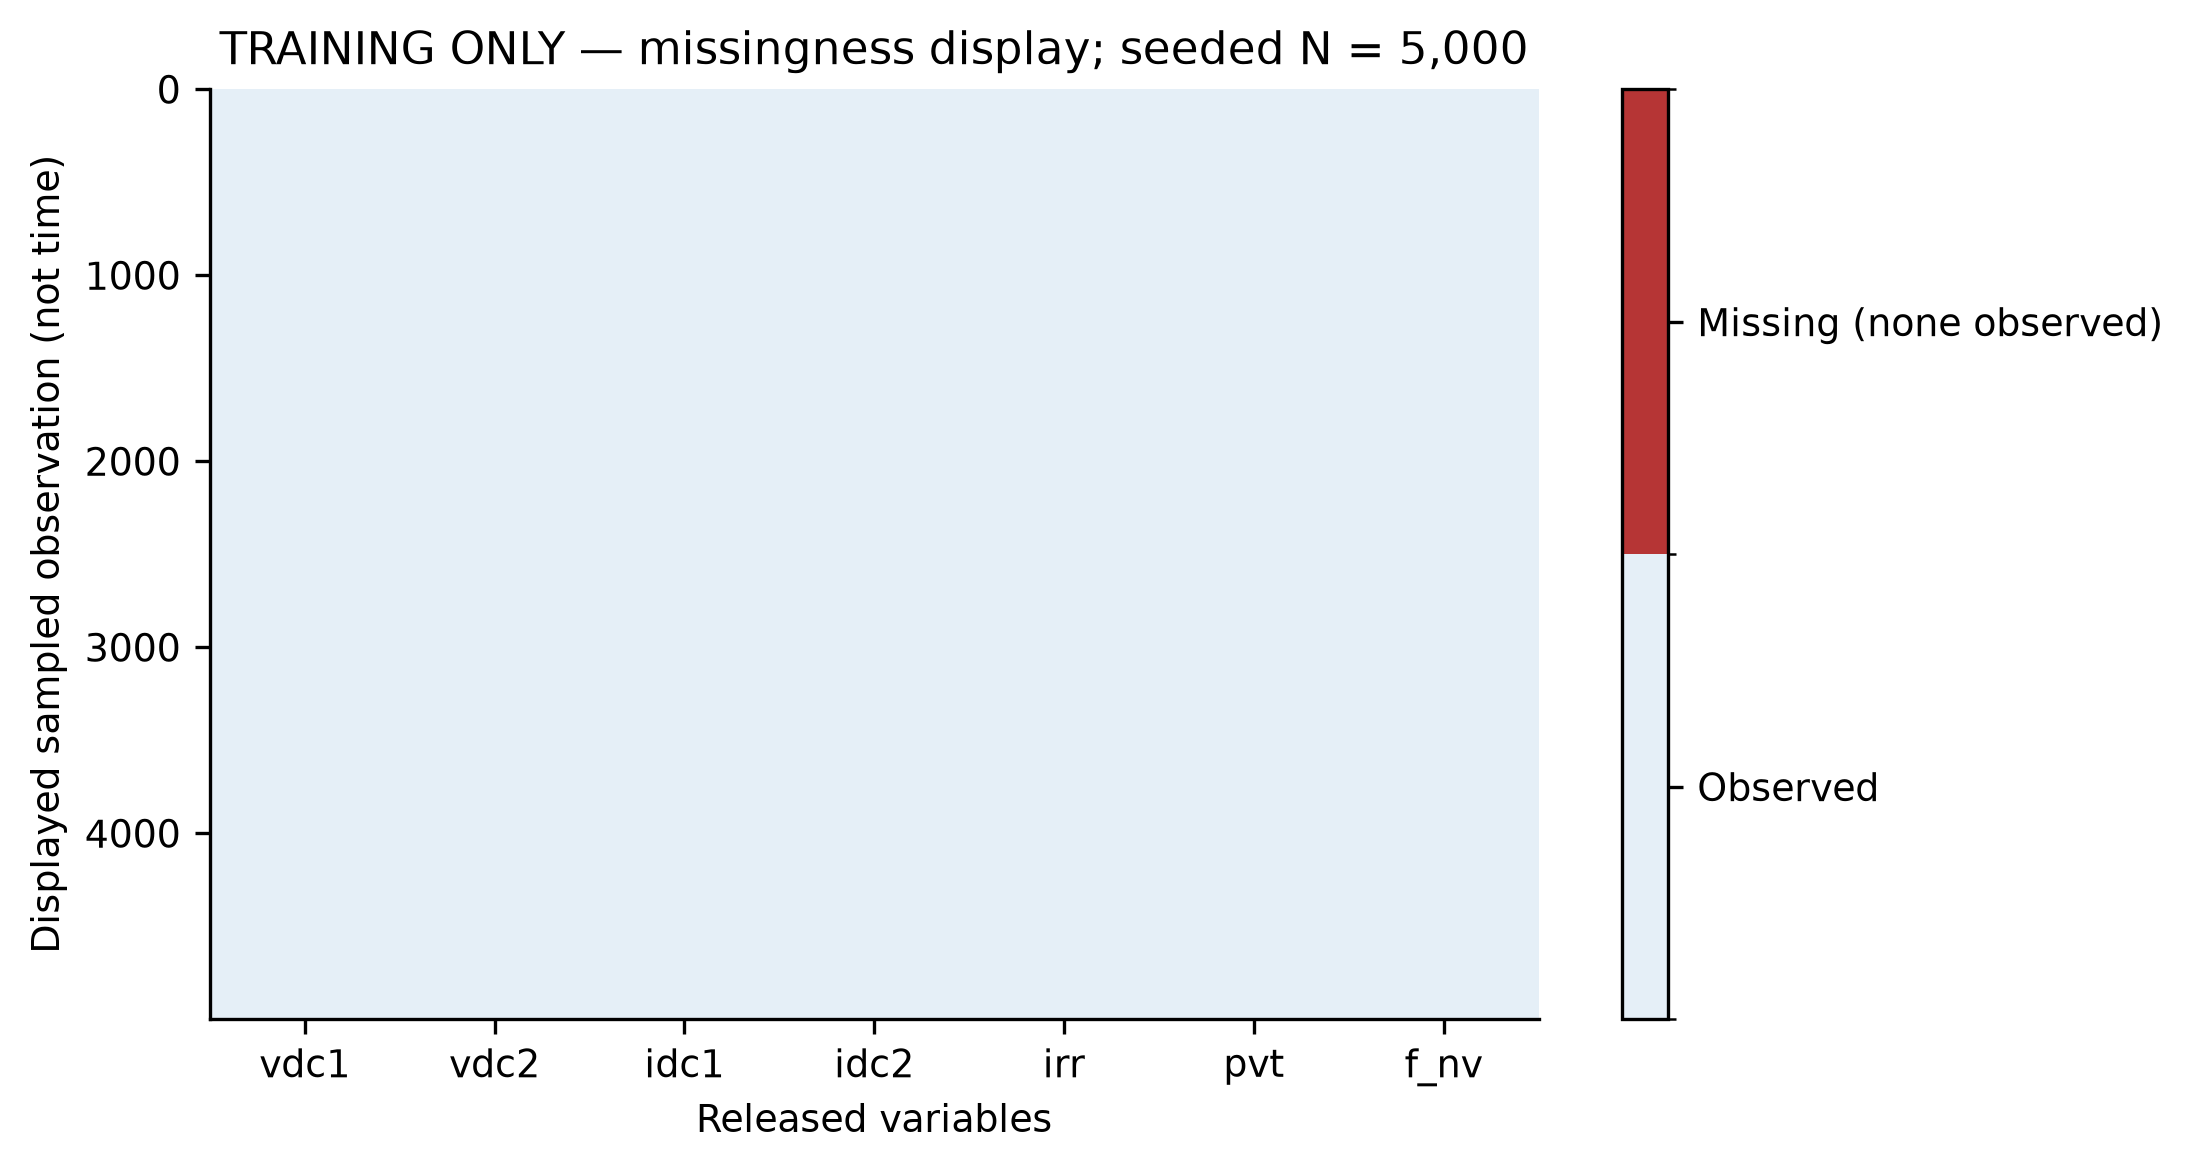
\includegraphics[width=0.98\textwidth,height=0.62\textheight,keepaspectratio]{../../figures/fig1_1_missingness_heatmap.png}
\caption{Missingness pattern: seed-42 uniform TRAIN display, N=5,000. Full-export conventional missingness is 0/9,616,586 cells; the 62 paired zeros remain observations.}\label{fig:missing}
\end{figure*}
\begin{figure*}[!t]
\centering
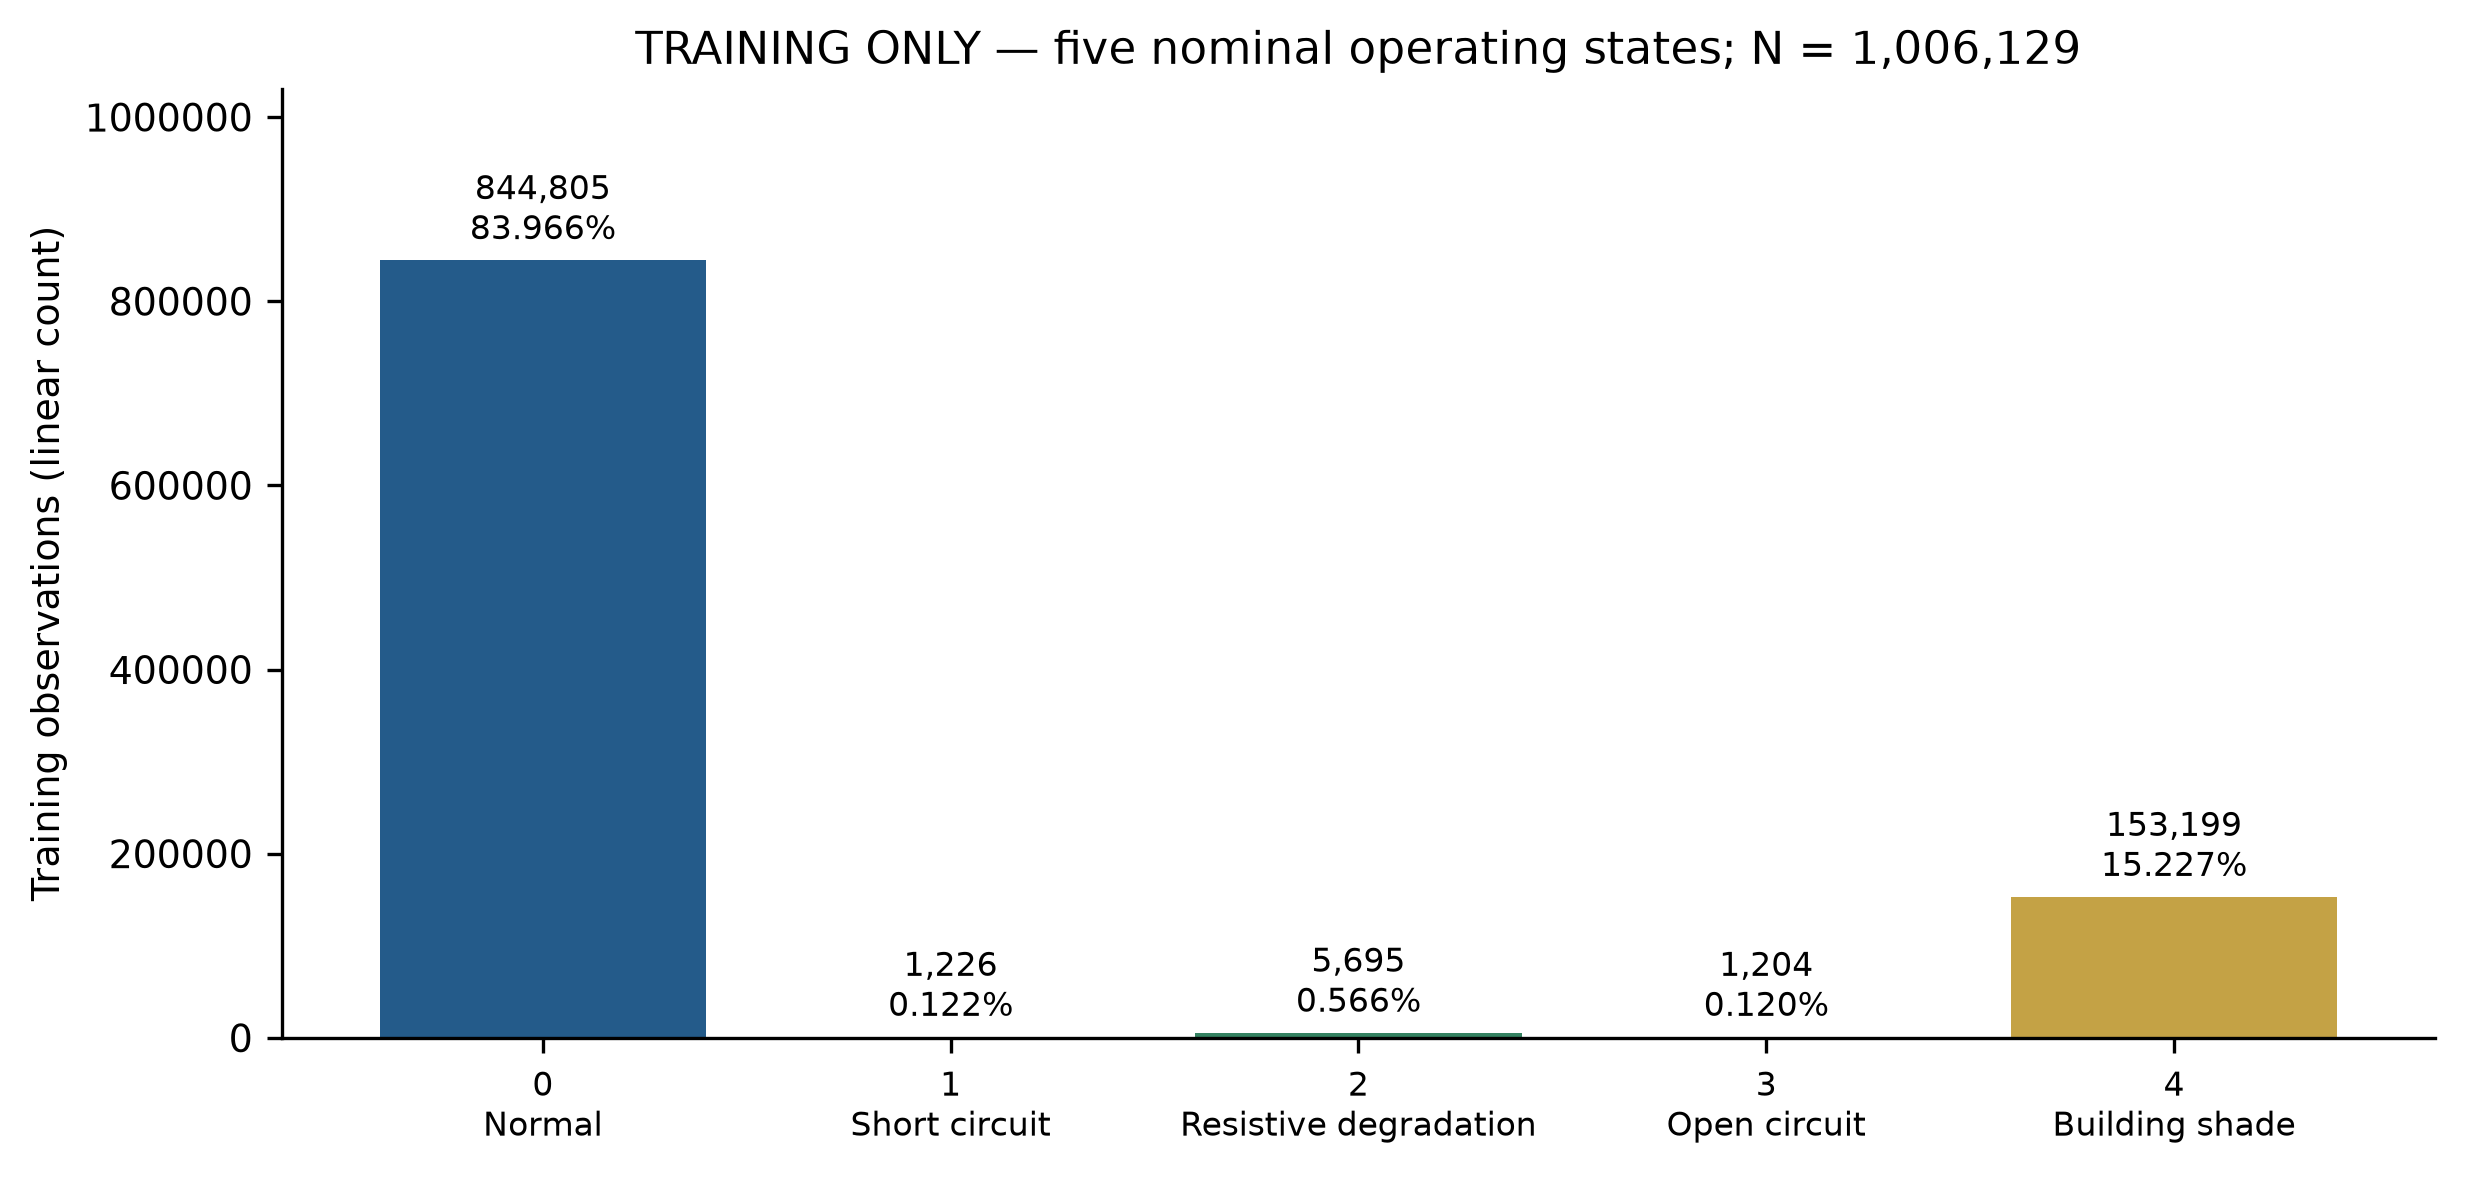
\includegraphics[width=0.98\textwidth,height=0.62\textheight,keepaspectratio]{../../figures/fig1_2_target_distribution.png}
\caption{Target distribution: all 1,006,129 TRAIN positions, unchanged nominal class labels and natural prevalence. Normal contributes approximately 83.966\%; no resampling is applied.}\label{fig:target}
\end{figure*}
\begin{figure*}[!t]
\centering
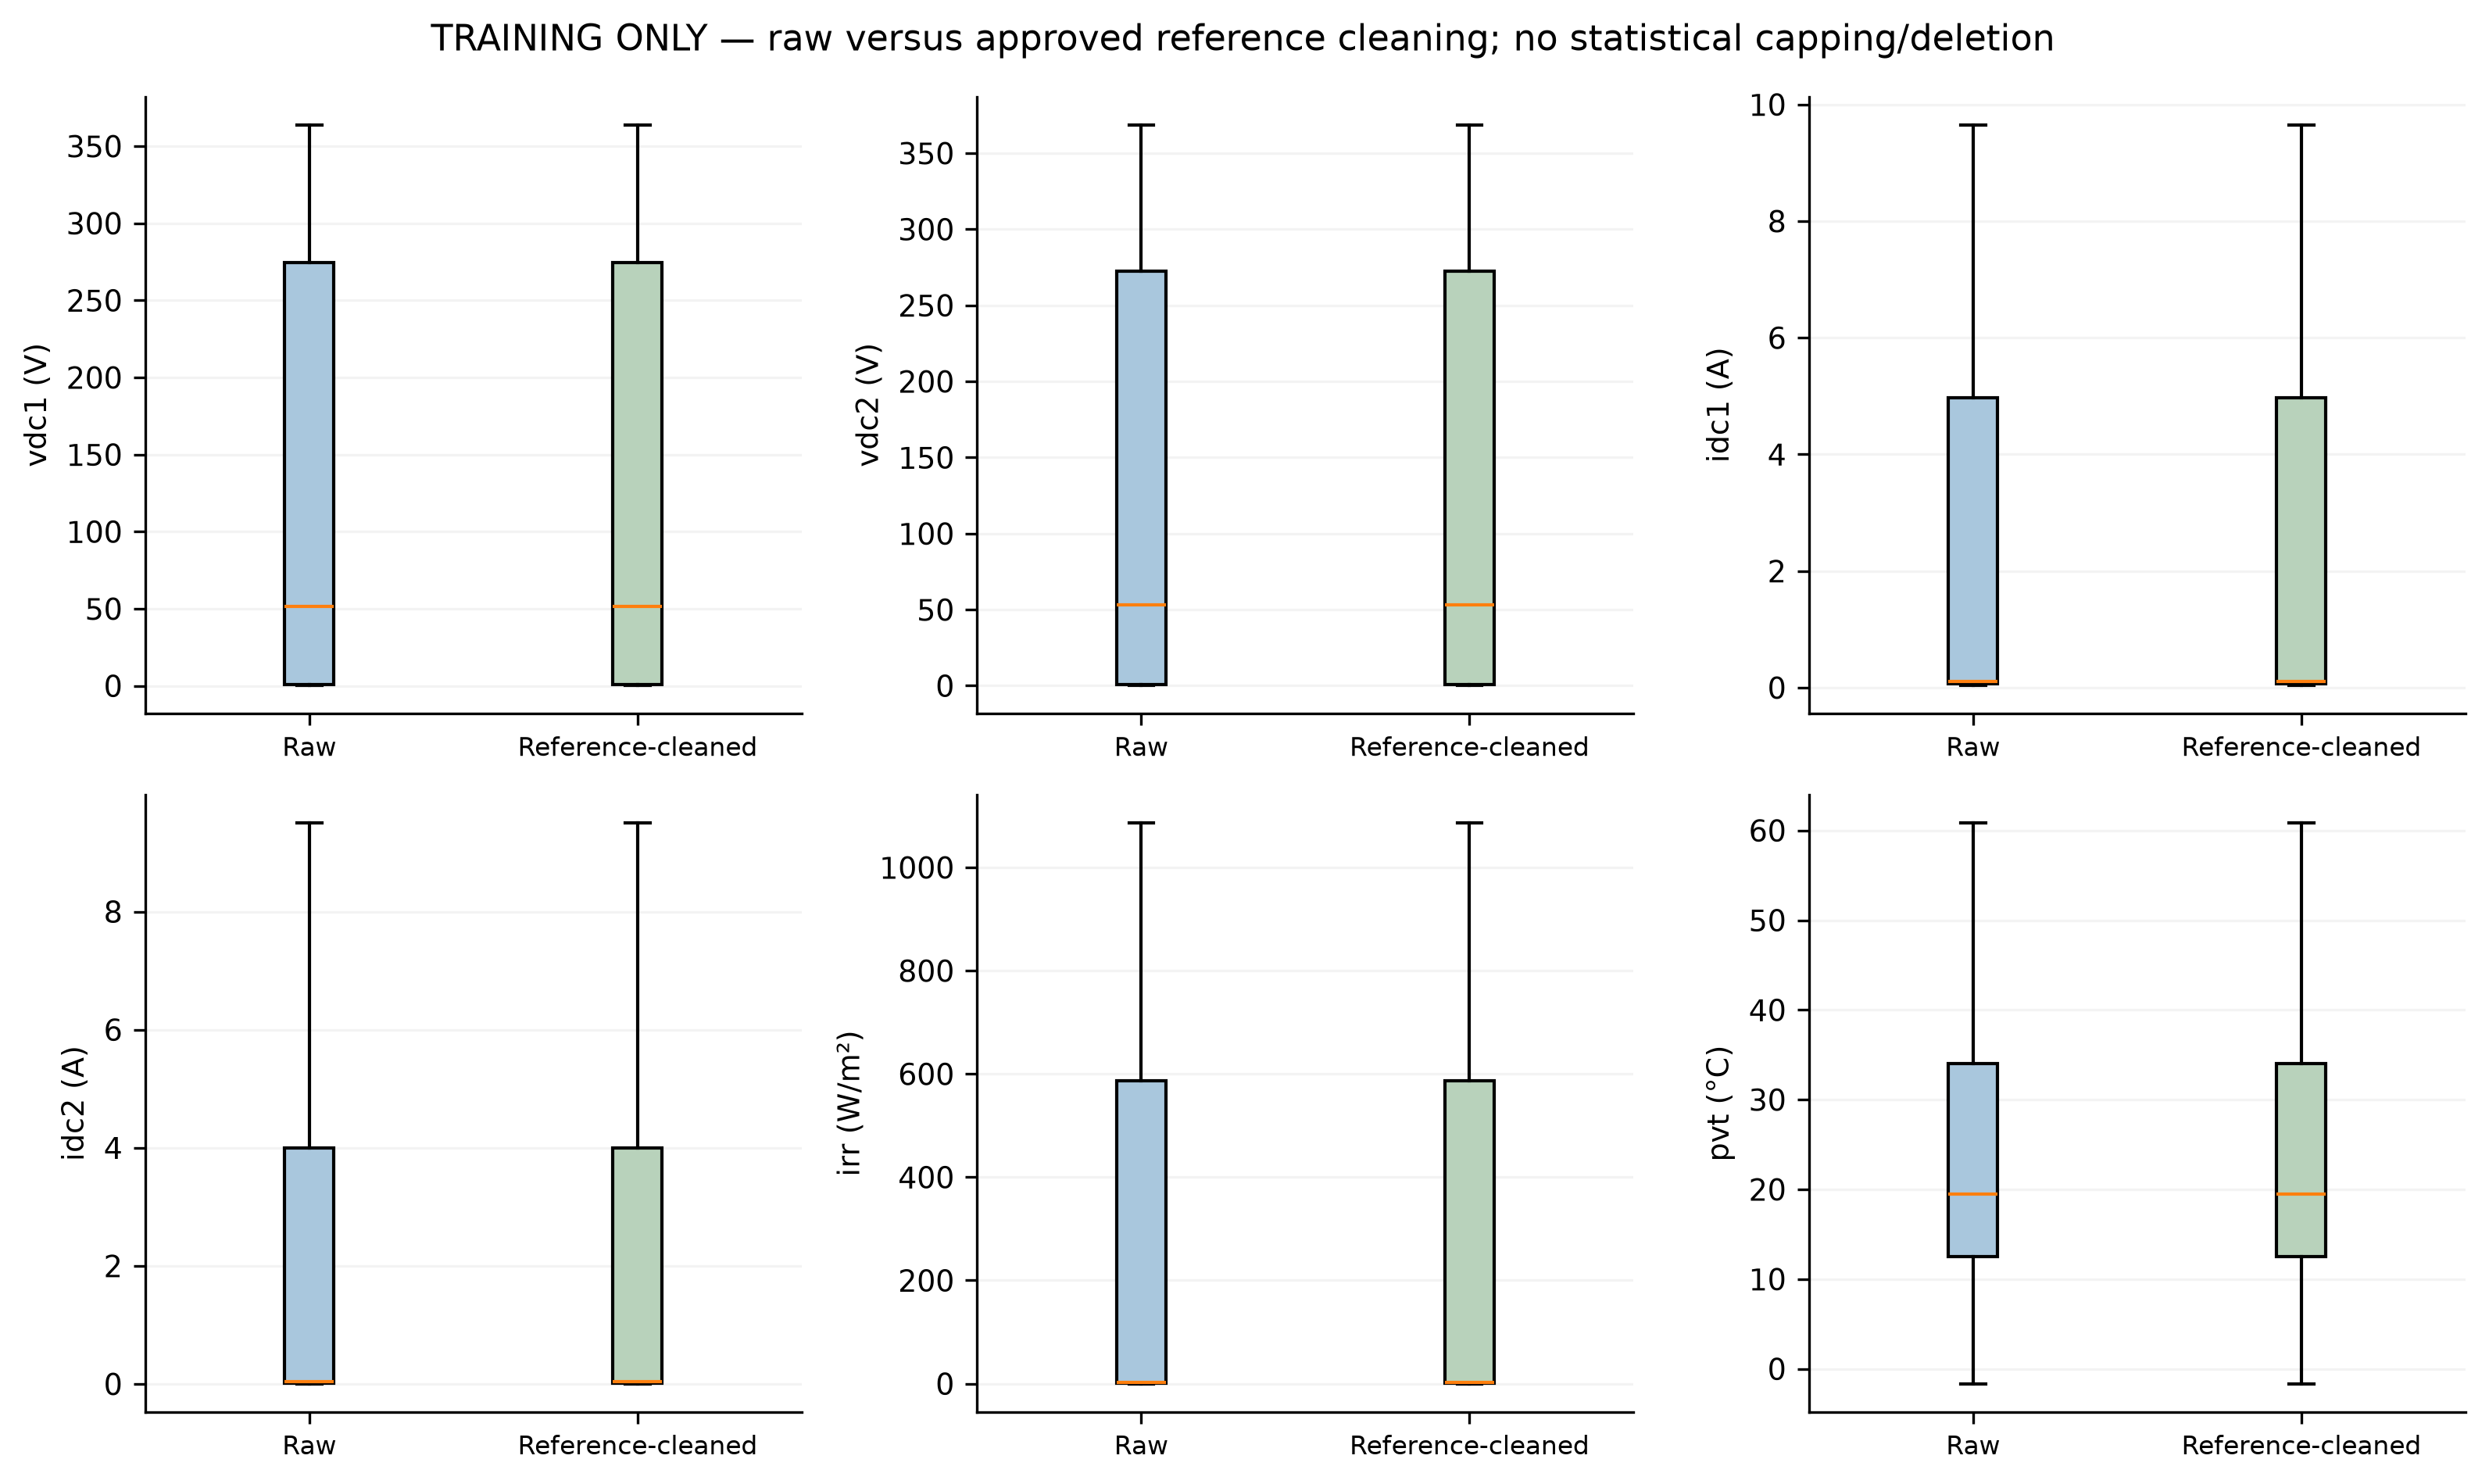
\includegraphics[width=0.98\textwidth,height=0.62\textheight,keepaspectratio]{../../figures/fig2_1_outlier_boxplots.png}
\caption{TRAIN raw versus reference-cleaned boxplots with IQR whiskers and retained observations. No statistical capping or deletion is selected; zero outside-fence flags reflect the actual full-TRAIN screen, not physical certification.}\label{fig:outliers}
\end{figure*}
\begin{figure*}[!t]
\centering
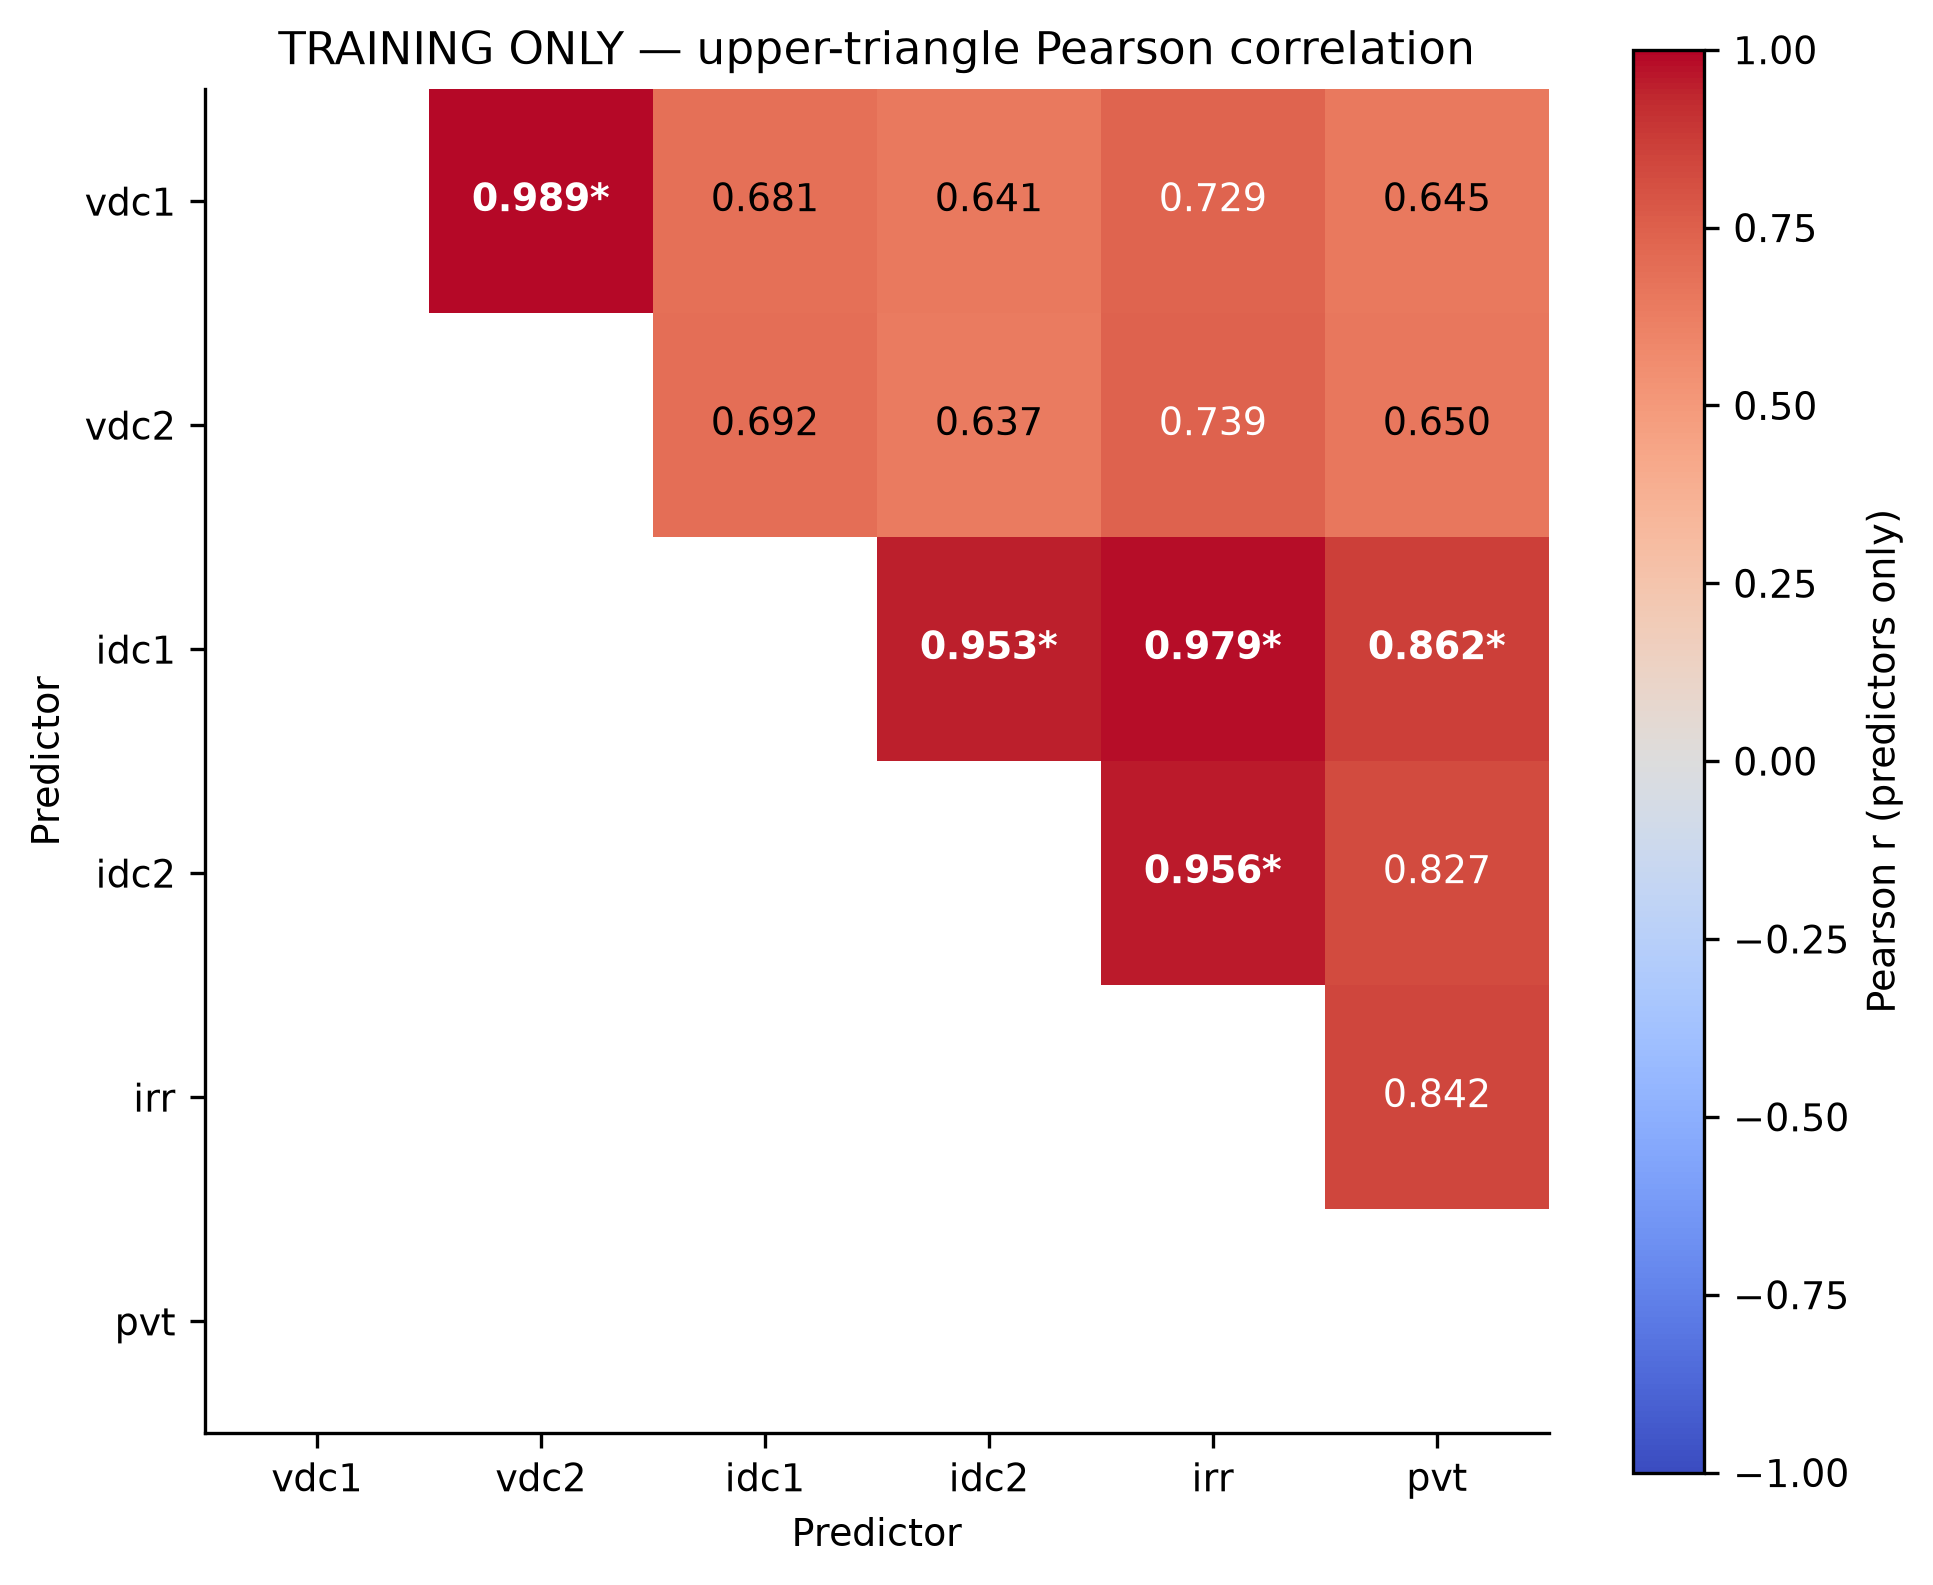
\includegraphics[width=0.98\textwidth,height=0.62\textheight,keepaspectratio]{../../figures/fig3_1_correlation_matrix.png}
\caption{TRAIN predictor-only upper-triangle Pearson correlation. Five pairs satisfy $|r|\geq0.85$; f\_nv is excluded. Warning thresholds do not automatically remove physical measurements.}\label{fig:correlation}
\end{figure*}
\begin{figure*}[!t]
\centering
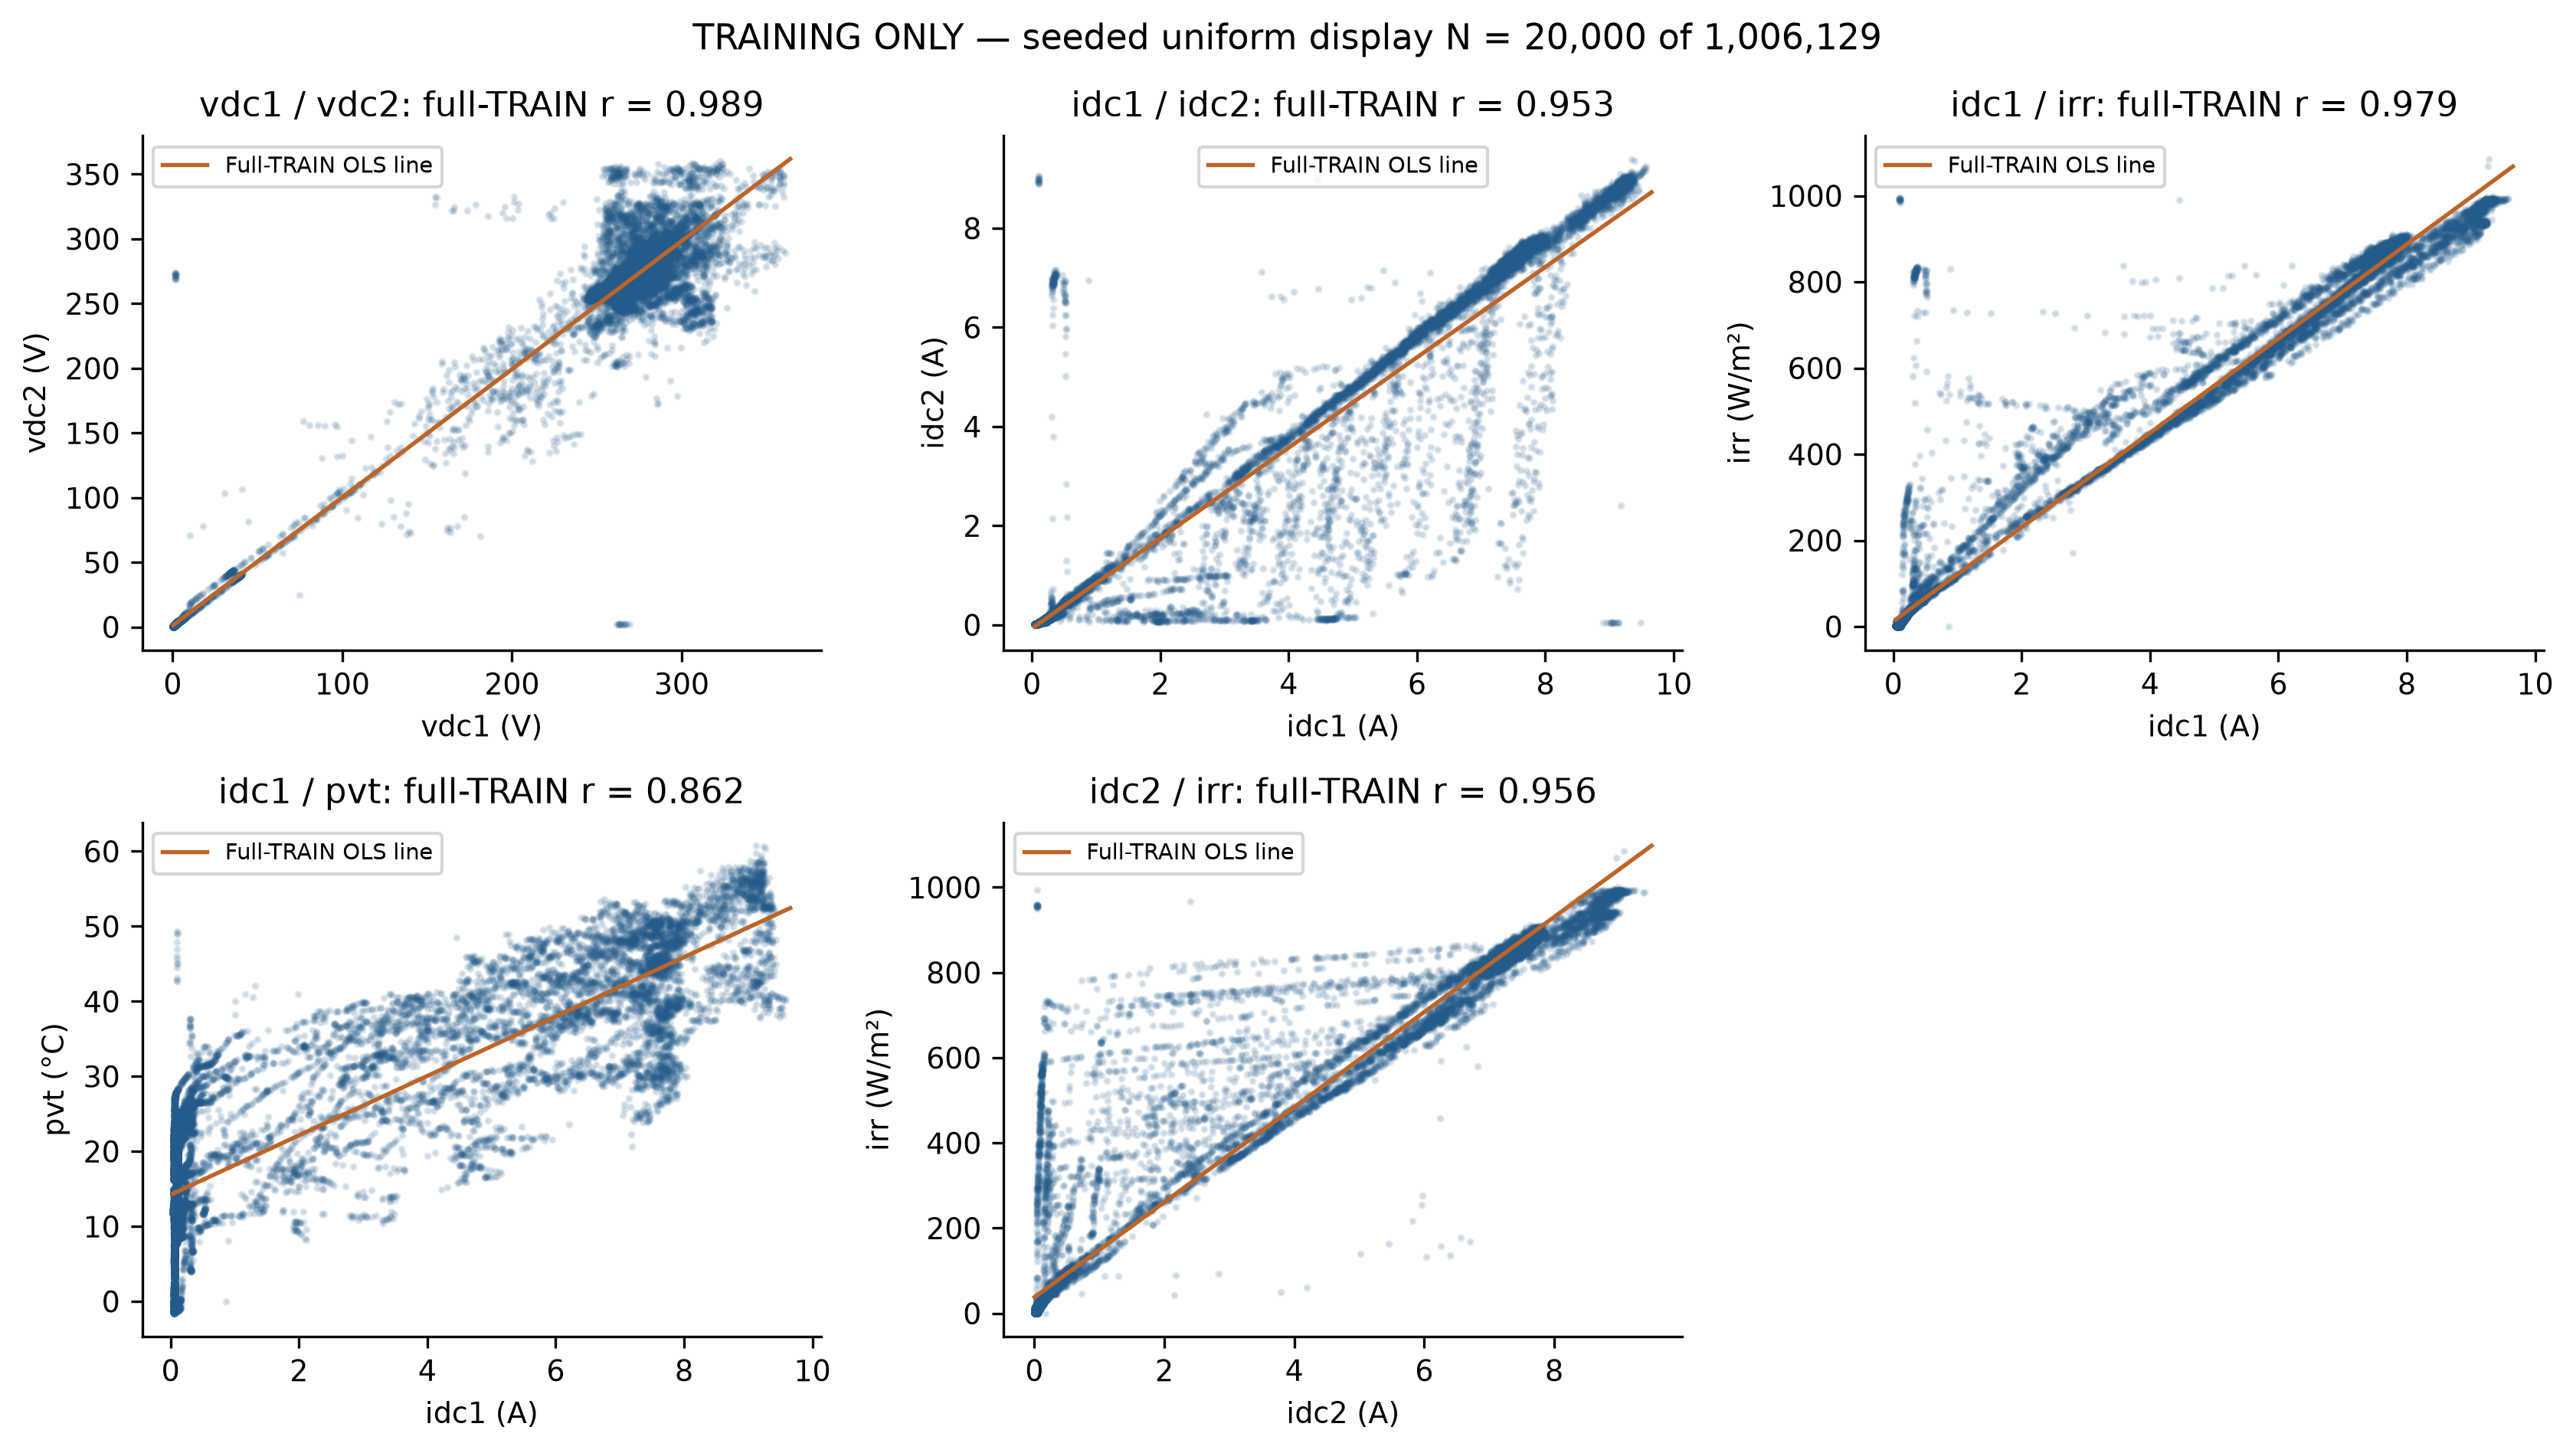
\includegraphics[width=0.98\textwidth,height=0.62\textheight,keepaspectratio]{../../figures/fig3_2_collinear_scatterplots.png}
\caption{All five collinear pairs. Seed-42 uniform TRAIN scatter display N=20,000; fitted descriptive lines and Pearson values use full TRAIN. Neither lines nor association imply causal or independent samples.}\label{fig:scatter}
\end{figure*}
\begin{figure*}[!t]
\centering
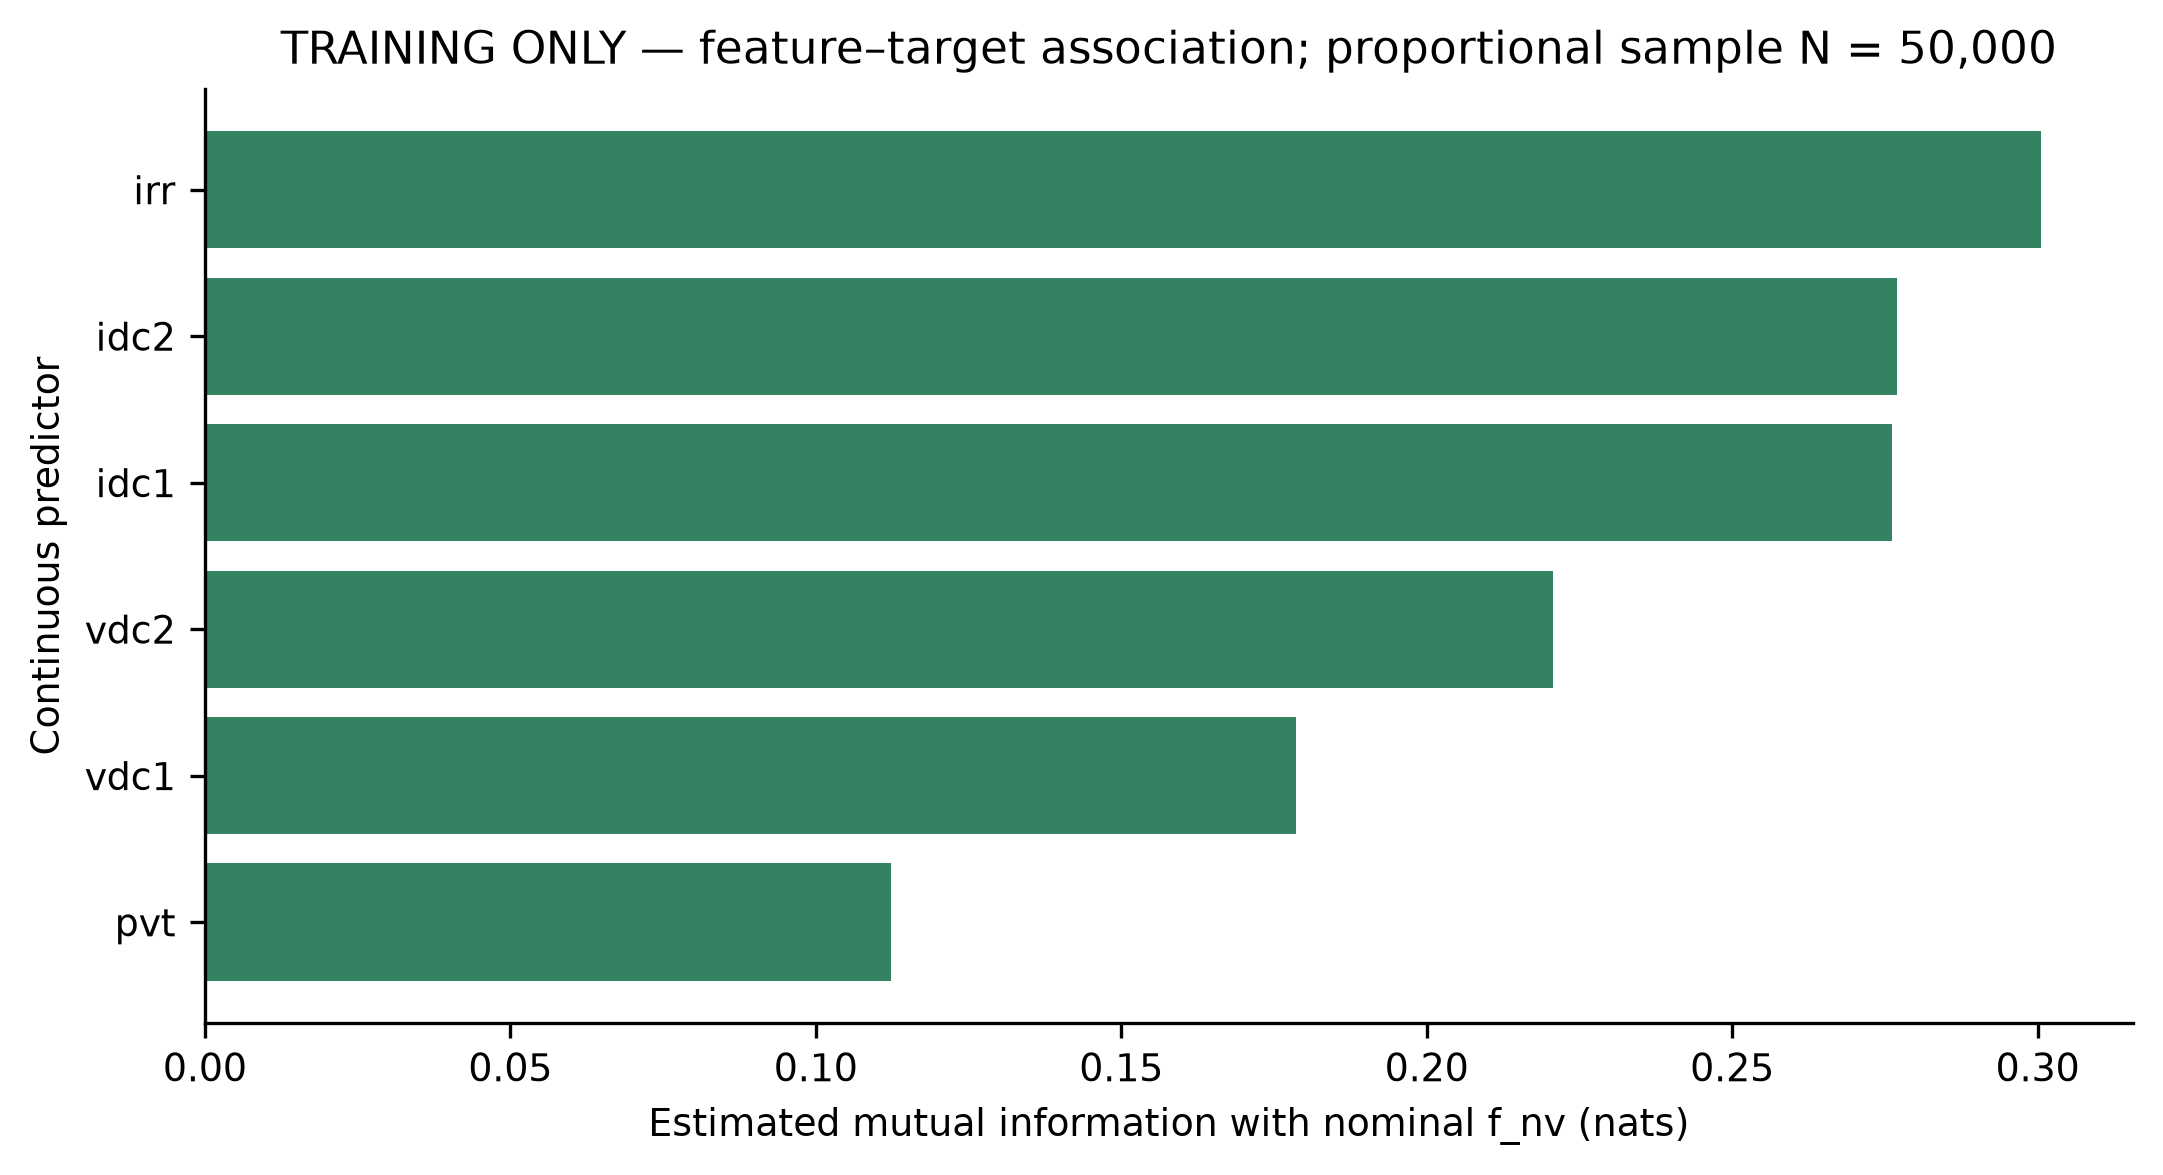
\includegraphics[width=0.98\textwidth,height=0.62\textheight,keepaspectratio]{../../figures/fig3_3_target_importance.png}
\caption{Target Association / Mutual Information Feature Screening. Continuous-predictor / nominal-target MI, seed 42, proportional TRAIN sample N=50,000, k=3. This is descriptive preprocessing relevance, not trained-model feature importance.}\label{fig:mi}
\end{figure*}
\begin{figure*}[!t]
\centering
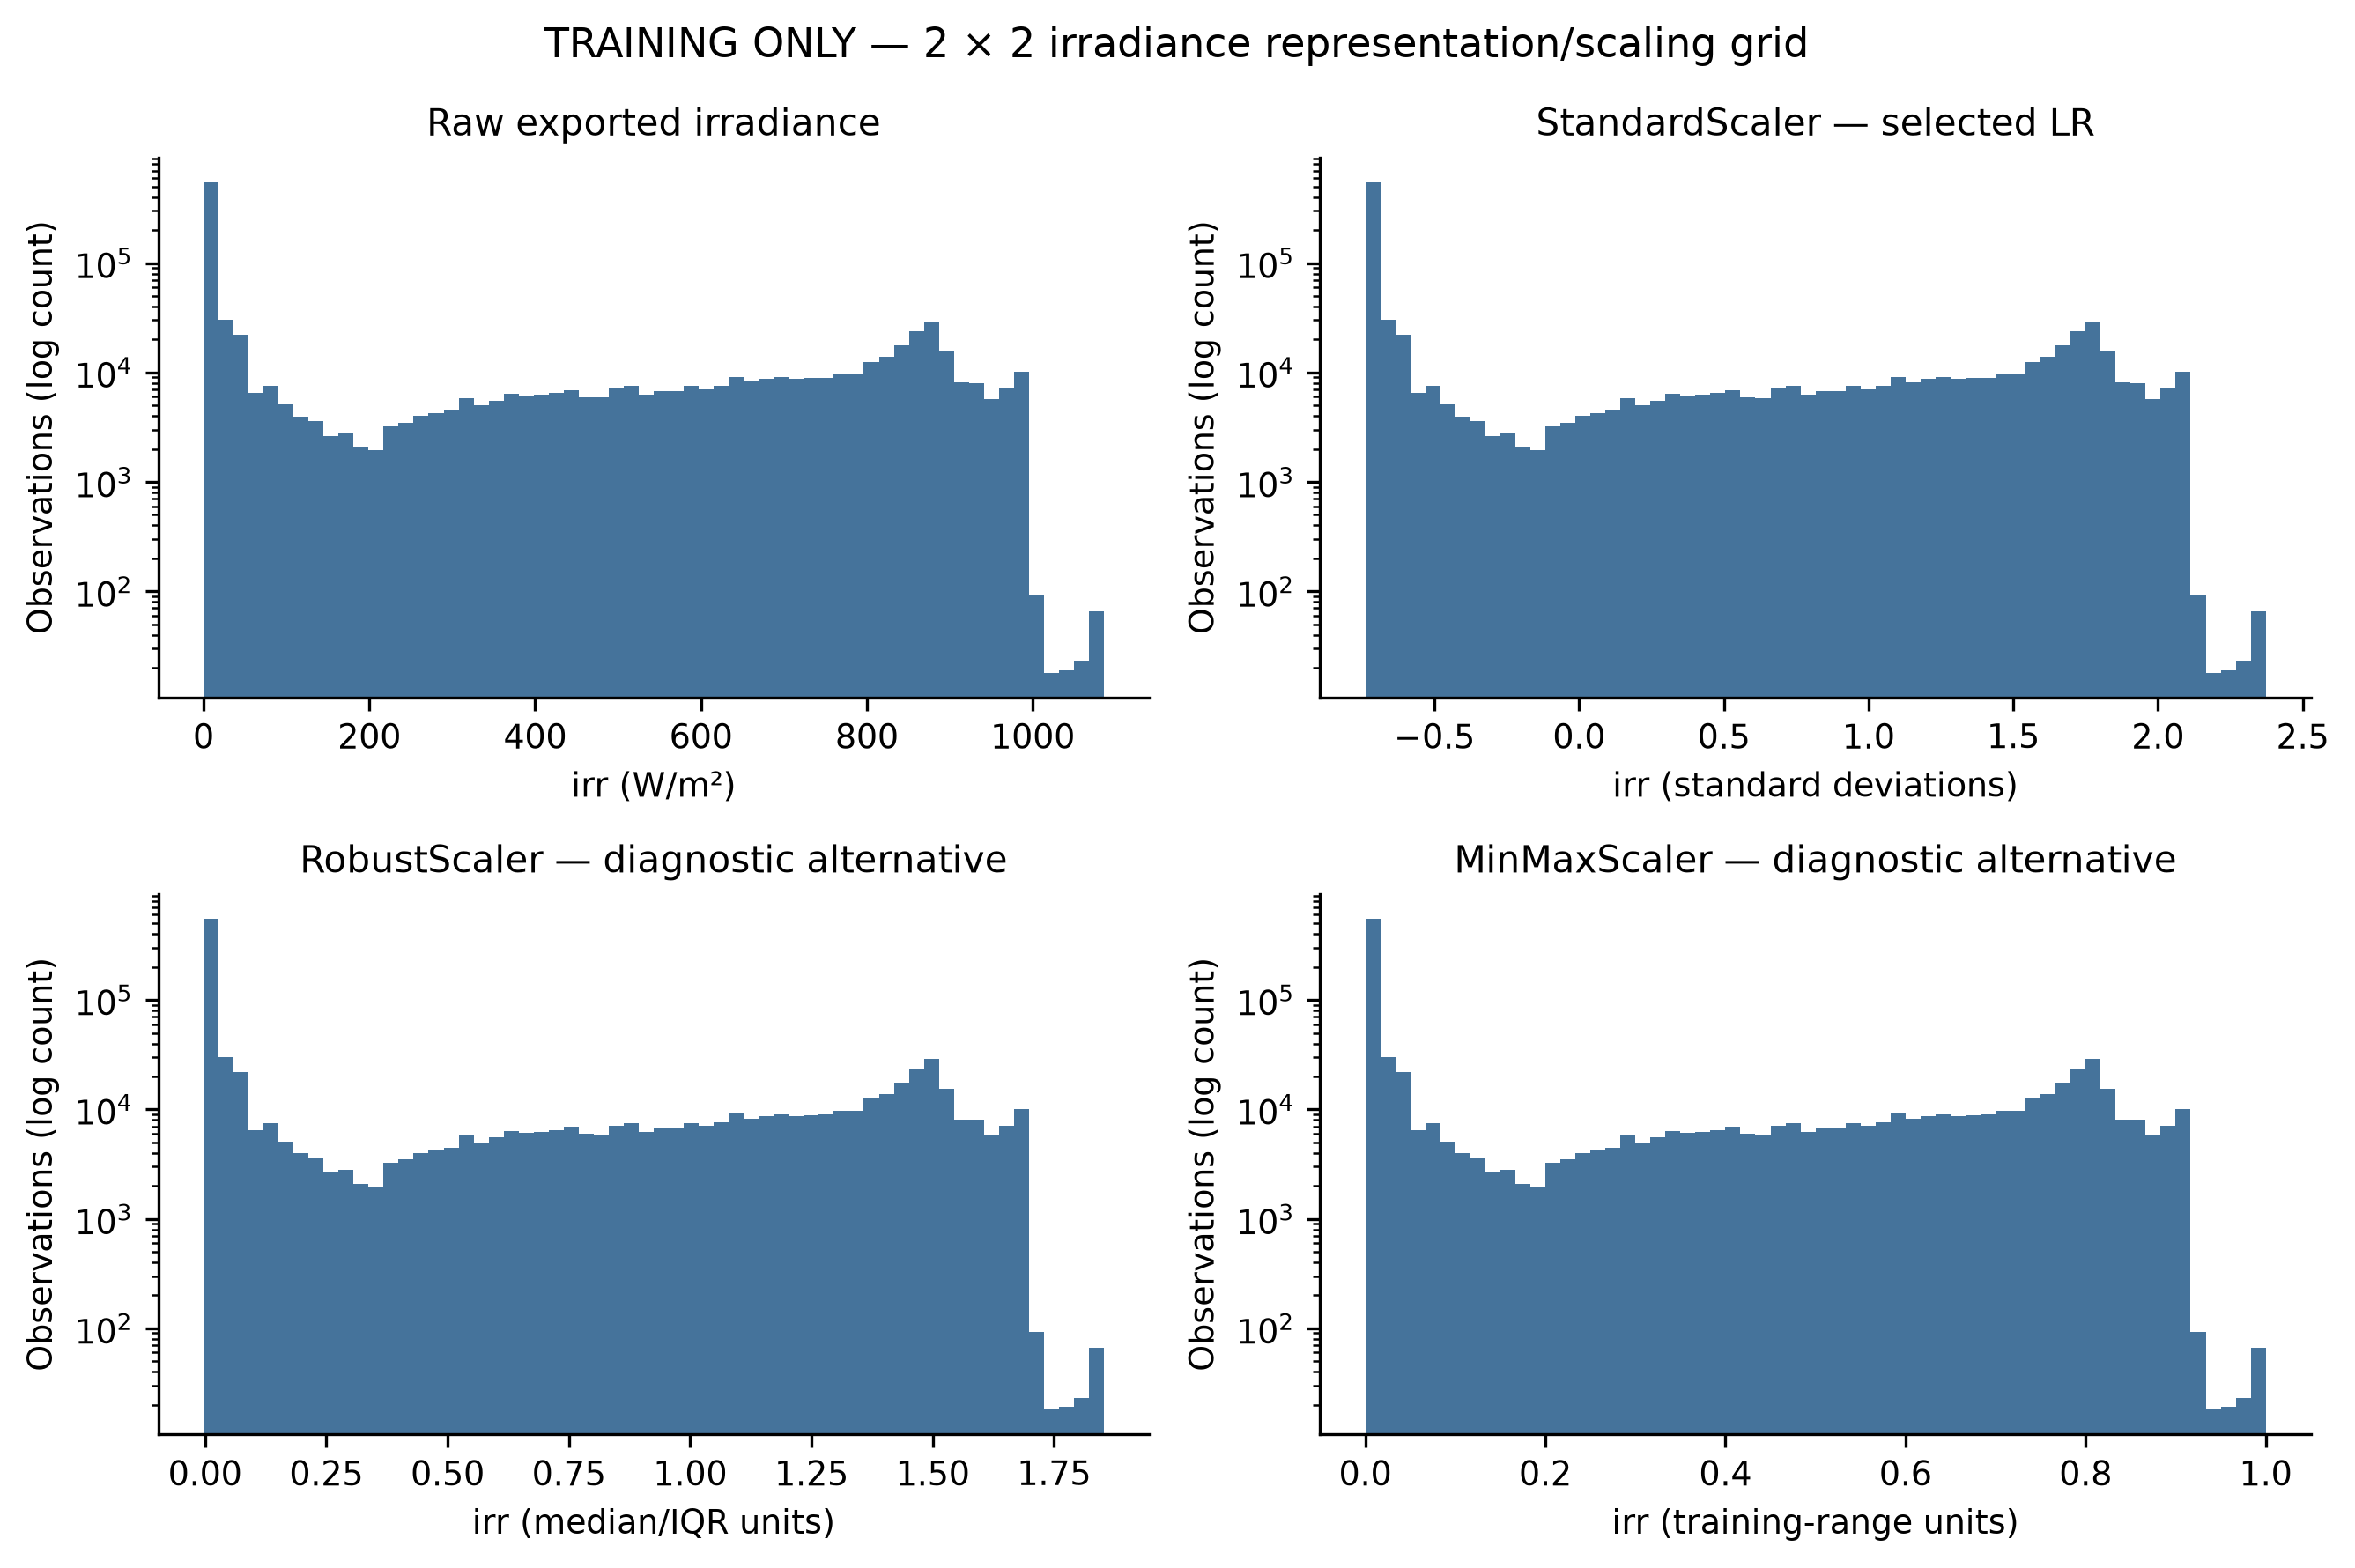
\includegraphics[width=0.98\textwidth,height=0.62\textheight,keepaspectratio]{../../figures/fig4_1_transformation_grid.png}
\caption{Original TRAIN transformation/scaling grid. StandardScaler is the reference standardized representation; Robust/MinMax are diagnostics. Original algorithm labels describe intended preprocessing rationale only. No log transform or downstream model-selection outcome is claimed.}\label{fig:scaling}
\end{figure*}
\begin{figure*}[!t]
\centering
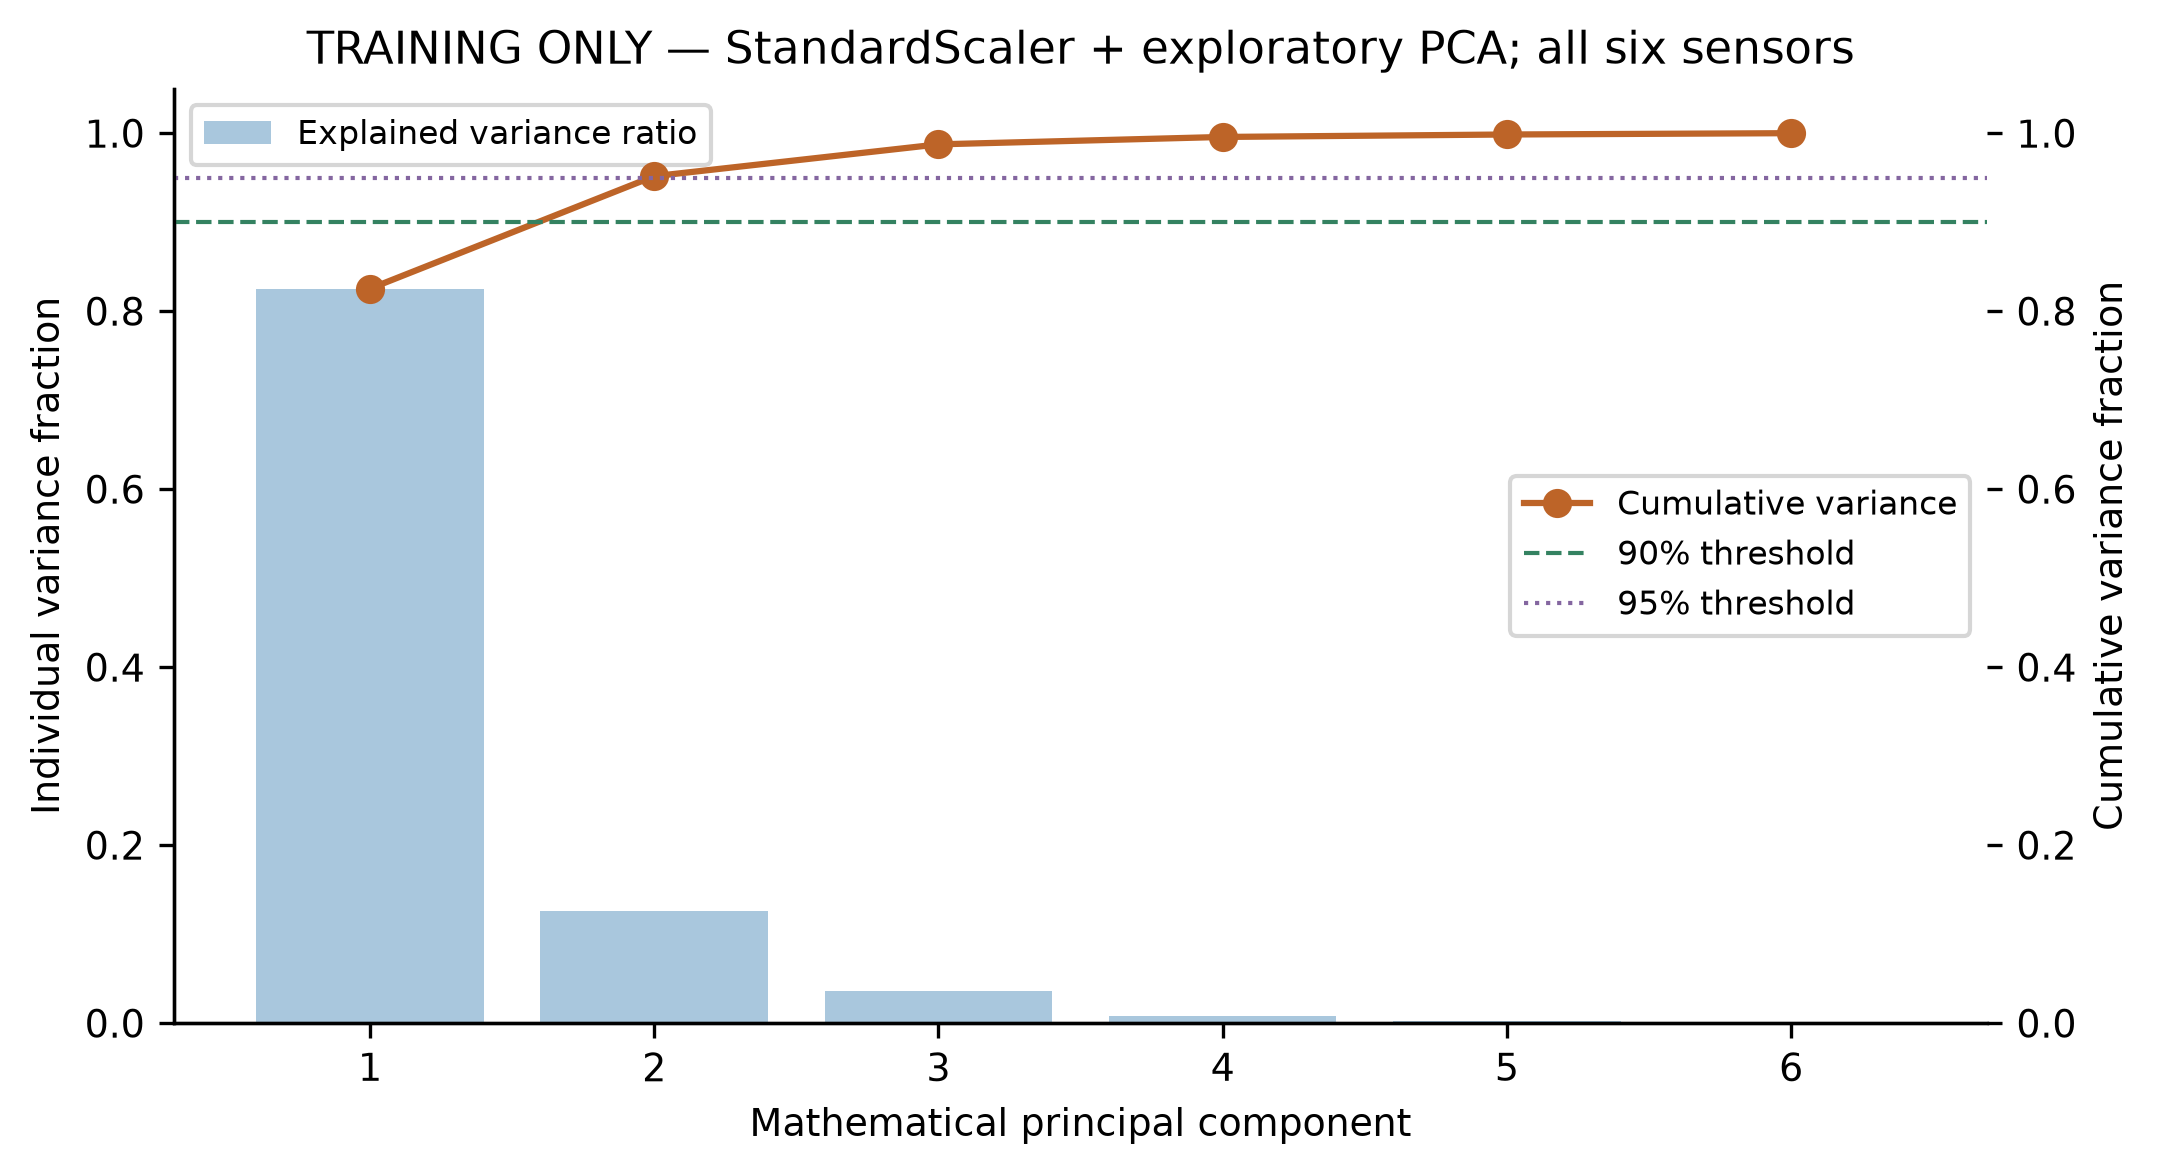
\includegraphics[width=0.98\textwidth,height=0.62\textheight,keepaspectratio]{../../figures/fig5_1_pca_scree_plot.png}
\caption{Exploratory StandardScaler--PCA fitted on full TRAIN only. Bars give individual variance, line cumulative variance, dashed/dotted lines 90\%/95\% cutoffs. Two components explain 95.1677\%, requiring all six physical inputs.}\label{fig:pca}
\end{figure*}

\clearpage
\begin{thebibliography}{00}
\bibitem{dataset} C. H. Costa, ``PV Fault Dataset,'' original-author repository, commit e9ed8ad8072dcb3ffc643b0f3604219798708551. [Online]. Available: \url{https://github.com/clayton-h-costa/pv_fault_dataset}. Original source README and Apache-2.0 license retained.
\bibitem{study} A. E. Lazzaretti et al., ``A monitoring system for online fault detection and classification in photovoltaic plants,'' \emph{Sensors}, vol. 20, no. 17, art. 4688, 2020, doi: 10.3390/s20174688.
\bibitem{phase1} R. Prince, ``Data preprocessing and feature engineering strategy,'' approved Phase 1 report and original audit evidence, Oct. 2026. Retained in \texttt{phase1\_strategy/}.
\bibitem{sklearn} Scikit-learn developers, ``Pipeline, ColumnTransformer, preprocessing, mutual\_info\_classif and PCA documentation.'' [Online]. Available: \url{https://scikit-learn.org/stable/}. Exact implementation versions are pinned in the repository.
\bibitem{ieee} IEEE, ``Manuscript templates for conference proceedings.'' [Online]. Available: \url{https://www.ieee.org/conferences/publishing/templates.html}. Unmodified IEEEtran v1.8b conference class distributed with report source; template provenance recorded separately.
\end{thebibliography}
\end{document}
